\documentclass [a4paper] {report}
\usepackage{amsmath,amssymb,amsthm, bbm, graphicx,listings,braket,subfig,titlesec,cleveref,lipsum,mcode,xcolor-patch, textcomp,float,booktabs,siunitx, listings}
\usepackage[authoryear]{natbib}
\usepackage[section]{placeins}
\usepackage[margin=2.2cm]{geometry}
\titleformat{\chapter}{\normalfont\huge}{\thechapter.}{20pt}{\huge \bf}

\DeclareMathOperator*{\argmin}{arg\,min}
\DeclareMathOperator*{\argmax}{arg\,max}
\newcommand{\norm}[1]{\left\lVert #1 \right\rVert}

\begin{document}
	
	\begin{titlepage}
		\begin{center}
			
			\textsc{\LARGE IN4320 Machine Learning}\\[1.25cm]
			
			\rule{\linewidth}{0.5mm}\\[1.0cm]
			{\huge \bfseries Exercises: Semi-Supervised Learning }\\[0.6cm]
			\rule{\linewidth}{0.5mm}\\[1.5cm]
			
			\begin{minipage}{0.4\textwidth}
				\begin{flushleft} \large	
					\emph{Author:}\\
					\textsc{Milan Niestijl, 4311728}
				\end{flushleft}
			\end{minipage}
			
			\vfill
			{\large \today}
		\end{center}
	\end{titlepage}
	
	\section*{a.}
	In these exercises, two different methods of doing semi-supervised learning on a two-class LDA classifier are investigated. We now describe both methods on an algorithmic level. Recall that the probability density function in two-class LDA is given by:
	$$ f(x,y| \pi_{1}, \pi_{2}, \mu_{1},\mu_{2}, \Sigma) = \pi_{1}\mathcal{N}(x|\mu_{1}, \Sigma)\mathbbm{1}_{y=1} + \pi_{2}\mathcal{N}(x|\mu_{2}, \Sigma)\mathbbm{1}_{y=2}$$
	Where $\pi_{1}, \pi_{2} \in [0,1]: \pi_{1} + \pi_{2} =1$ and $\mathcal{N}(x|\mu, \Sigma)$ corresponds to the probability density function of a normal distribution with mean $\mu$ and covariance $\Sigma$.
	\subsection*{Supervised LDA}
	The maximum likelihood solution of the supervised problem can be shown to be given by:
	\begin{align*}
		\pi_{i} &= {1 \over N} \sum_{n=1}^{N}x_{n}\mathbbm{1}_{\{y_{n}=i\}}\\
		\mu_{i} &= \frac{\sum_{n=1}^{N}x_{n}\mathbbm{1}_{\{y_{n}=i\}}}{\sum_{n=1}^{N}\mathbbm{1}_{\{y_{n}=i\}}}\\
		\Sigma &= {1 \over N} \sum_{n=1}^{N} \left( x_{n} - \mu_{y_{n}} \right)\left( x_{n} - \mu_{y_{n}} \right)^{T}
	\end{align*}
	Where $x_{i}$ and $y_{i}$ denote the feature-values and label of the $i^{\text{th}}$ training sample.

	\subsection*{Self-Training}
	The first method of extending the supervised learner to a semi-supervised setting is called 'Self-Training', which first fits LDA using only the labelled data and then iteratively assigns the predicted label to unlabelled data if the confidence is bigger than a certain threshold (set to 0.7). In pseudo-code:
	
	\begin{lstlisting}
def fit_with_Self_training(X,y, max_iterations=100, treshold=0.7)
	counter = 0
	repeat {
		fit LDA on labelled data
		if (counter==max_iterations or no unlabelled data){
			break
		}
		predict labels of unlabelled data
		foreach point in unlabelled data do {
			if (confidence>treshold):
				label point as predicted
		}		
	}
	self.covariance, self.means = result (TODO)
	\end{lstlisting}
	\subsection*{Label-Propagation}
	The second method is called 'Label-propagation' \citep{propagation}, which first defines a graph on the data by specifying the weights of all edges. There are multiple ways to do this, but in our case the weight $w_{ij}$ is given by $w_{ij} = \mathbbm{1}_{kNN(x_{j})}(x_{i})$. That is, the weight of the edge connecting point $i$ to point $j$ is $1$ if $i$ is one of the k-nearest neighbours of $j$ and $0$ otherwise. Next, a transition matrix $T$ is defined by 
	$$T_{ij} = \mathbb{P}(j \to i) = {w_{ij} \over \sum_{k} w_{kj} } $$
	We define a label matrix $Y$, where the $i^{\text{th}}$ row represents the probability distribution over the different classes for the $i^{\text{th}}$ data point. The propagation algorithm is shown below:
	\begin{lstlisting}[escapeinside={(*}{*)}]
	repeat untill convergence {
		1. propagate: (* $Y = TY$ *)
		2. Row-normalize (*$Y.$*)
		3. Clamp the labelled data: (* $Y_{ic} = \delta(y_{i}, c) $*)	
	}
	\end{lstlisting}
	So that the corresponding semi-supervised LDA algorithm is given by the following pseudo code:
	\begin{lstlisting}
def fit_with_LabelPropagation(X,y, treshold=0.7)
	newLabels = labelPropagation(X,y)
	LDA.fit(X,newlabels)
	self.covariance, self.means = result (TODO)
	\end{lstlisting}
	
	\section*{b. and c.}
	The algorithm is tested on set \texttt{Spambase Data Set} from the UCI repository\footnote{See http://archive.ics.uci.edu/ml/machine-learning-databases/spambase/spambase.data}.
	First the features are standardized, i.e., they are rescaled to have unit variance. As training data, a subset of the dataset is used, containing 75 random samples from each class and a varying number of unlabelled data points. We test the various implementations on the training data. Repeating the experiment a total of 50 times, the mean of the training error and the log-likelihood of the labelled data is plotted against the number of unlabelled samples in the training data. The corresponding standard deviations are shown as error bars. The result can be seen in figures \ref{spambase_error} and \ref{spambase_likelihood}. We see that the error on the training data increases for increasing number of unlabelled samples. This is not necessarily unexpected, as this may happen if the assumptions of the model are not valid. That is, the data may not be well modelled by two Gaussian distributions (with equal covariance).

	\textbf{FOR SUPERVISED CLASSIFICATION, THE TRAINING ERROR IS NOT CONSTANT AS IT PREDICTS ON UNLABELLED SAMPLES TOO}\\
	\textbf{SHOULD ONLY PREDICT LABELLED SAMPLES RIGHT?}
	\\
	\begin{figure}[H]
		\begin{center}
			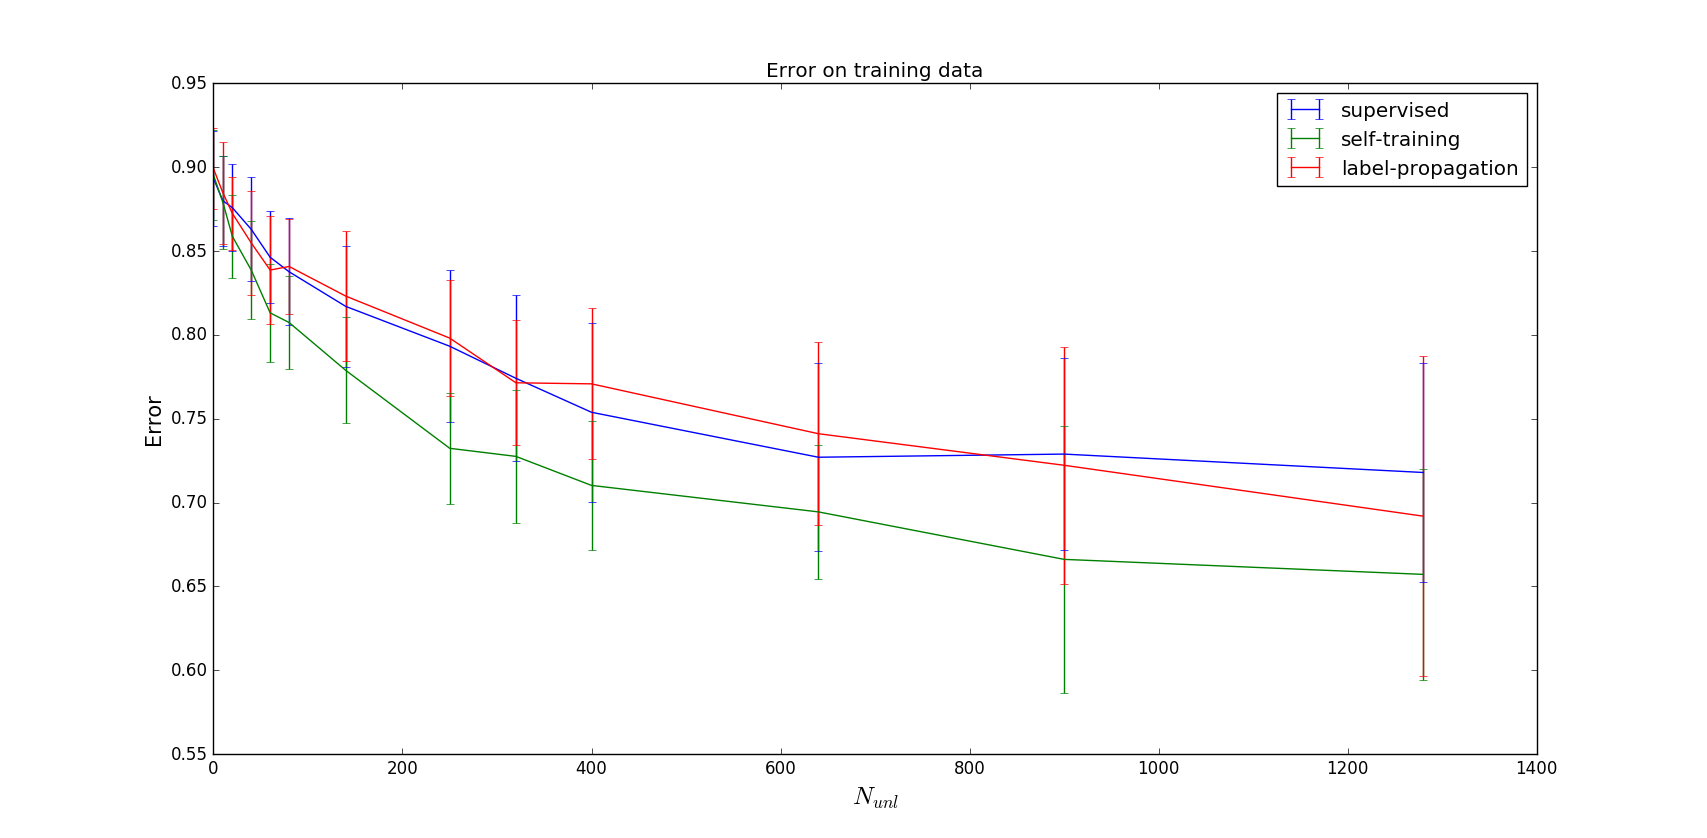
\includegraphics[scale=0.3]{Images/spambase_train_error.png}
			\caption{Error on the training data versus number of unlabelled samples, for various implementations of semi-supervised LDA.}
			\label{spambase_error}
		\end{center}
	\end{figure}

	\begin{figure}[H]
		\begin{center}
			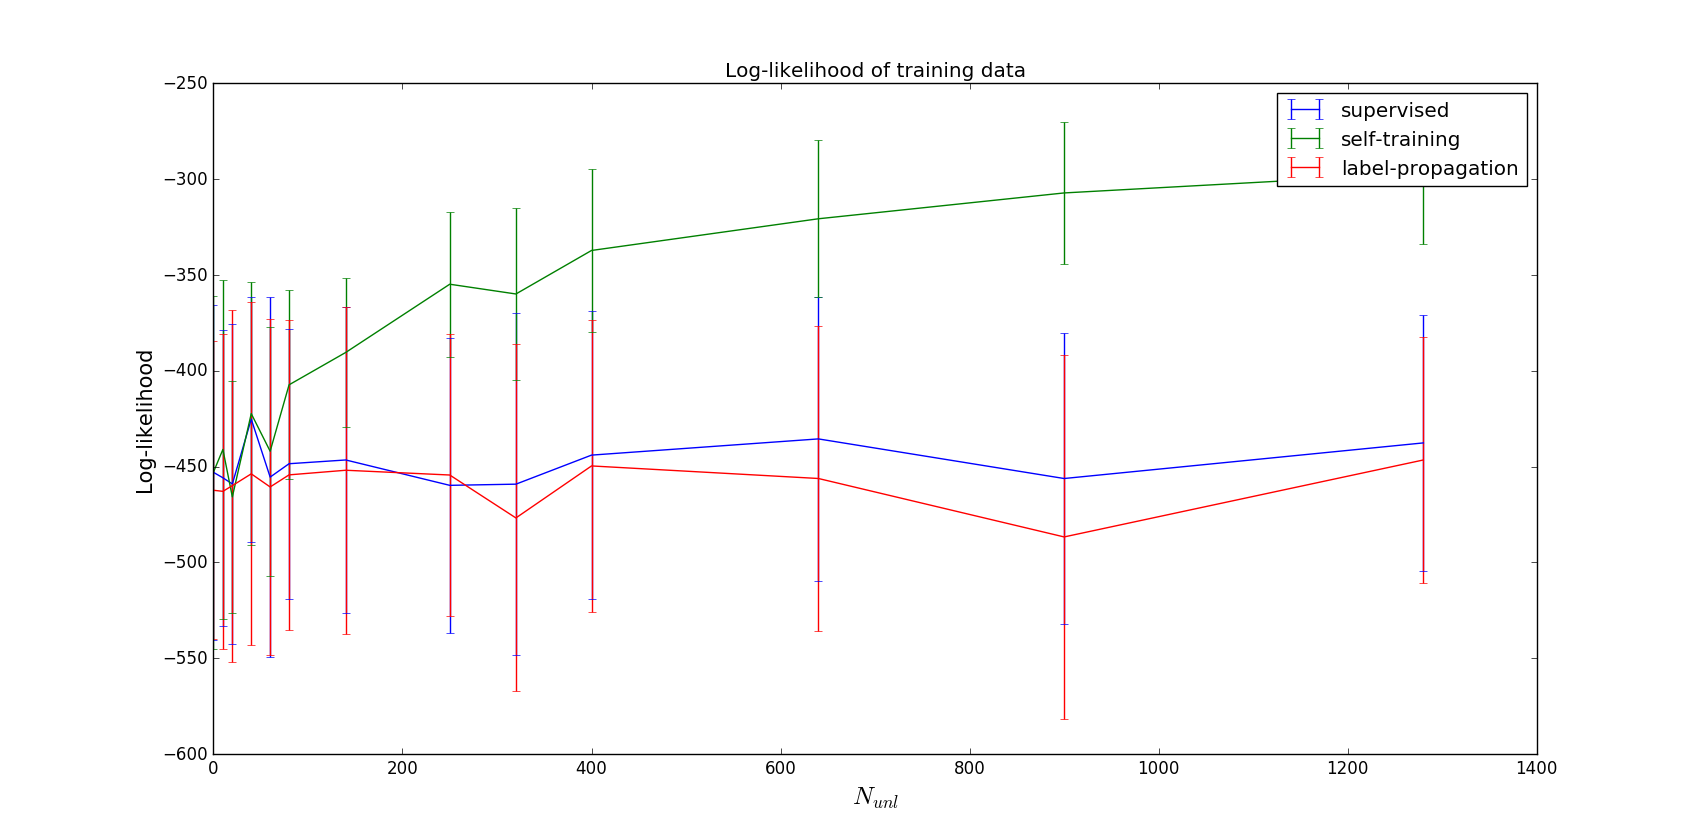
\includegraphics[scale=0.3]{Images/spambase_likelihood.png}
			\caption{Log-likelihood of the labelled samples in the training data versus number of unlabelled data points, for various implementations of semi-supervised LDA.}
			\label{spambase_likelihood}
		\end{center}
	\end{figure}
	
	\textbf{d.}
	We construct two datasets, such that the performance of one of the two methods for semi-supervised learning is worse than the supervised learner.\\
	\textbf{TODO: explanation of the distributions}\\
	A dataset drawn from the first custom distribution, along with the predictions of the various methods is shown in figure \ref{custom_1_dist}. It can be seen that the error on the training data get significantly worse for the self-training algorithm, whereas the label-propagation method performs similar to the supervised method. This is made even more clear in figure \ref{custom_1}, where the training error is plotted versus the number of unlabelled data.
	
	\begin{figure}[H]
		\begin{center}
			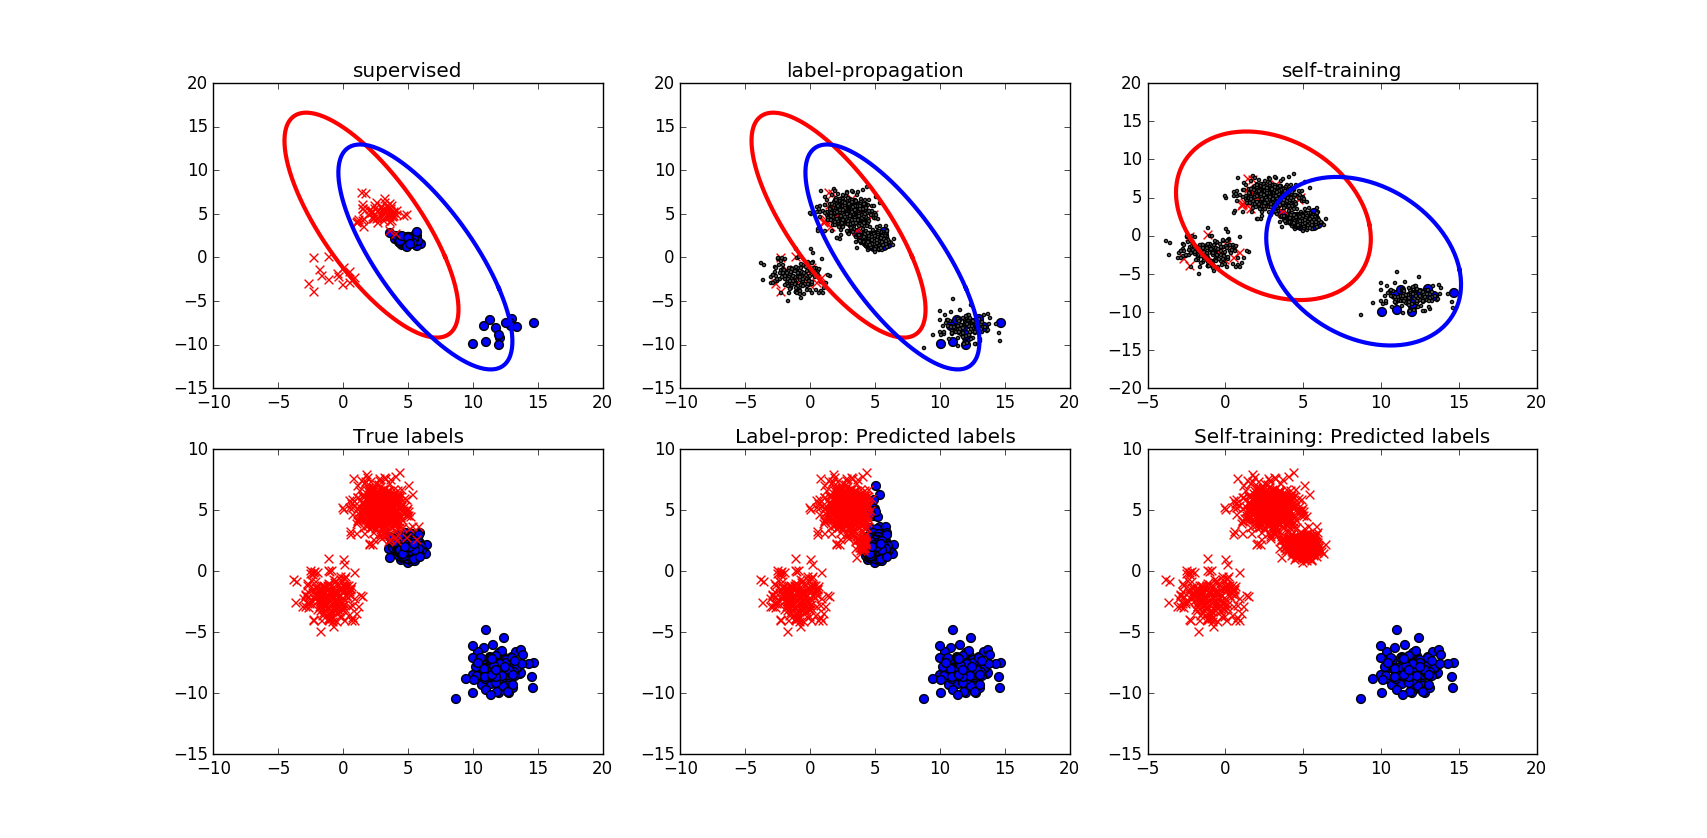
\includegraphics[scale=0.3]{Images/custom1.png}
			\caption{Distributions and predicted labels for various methods of semi-supervised LDA. The ellipses represent the covariance matrices of the normal distributions, centered around the corresponding mean.}
			\label{custom_1_dist}
		\end{center}
	\end{figure}	
	
	\begin{figure}[H]
		\begin{center}
			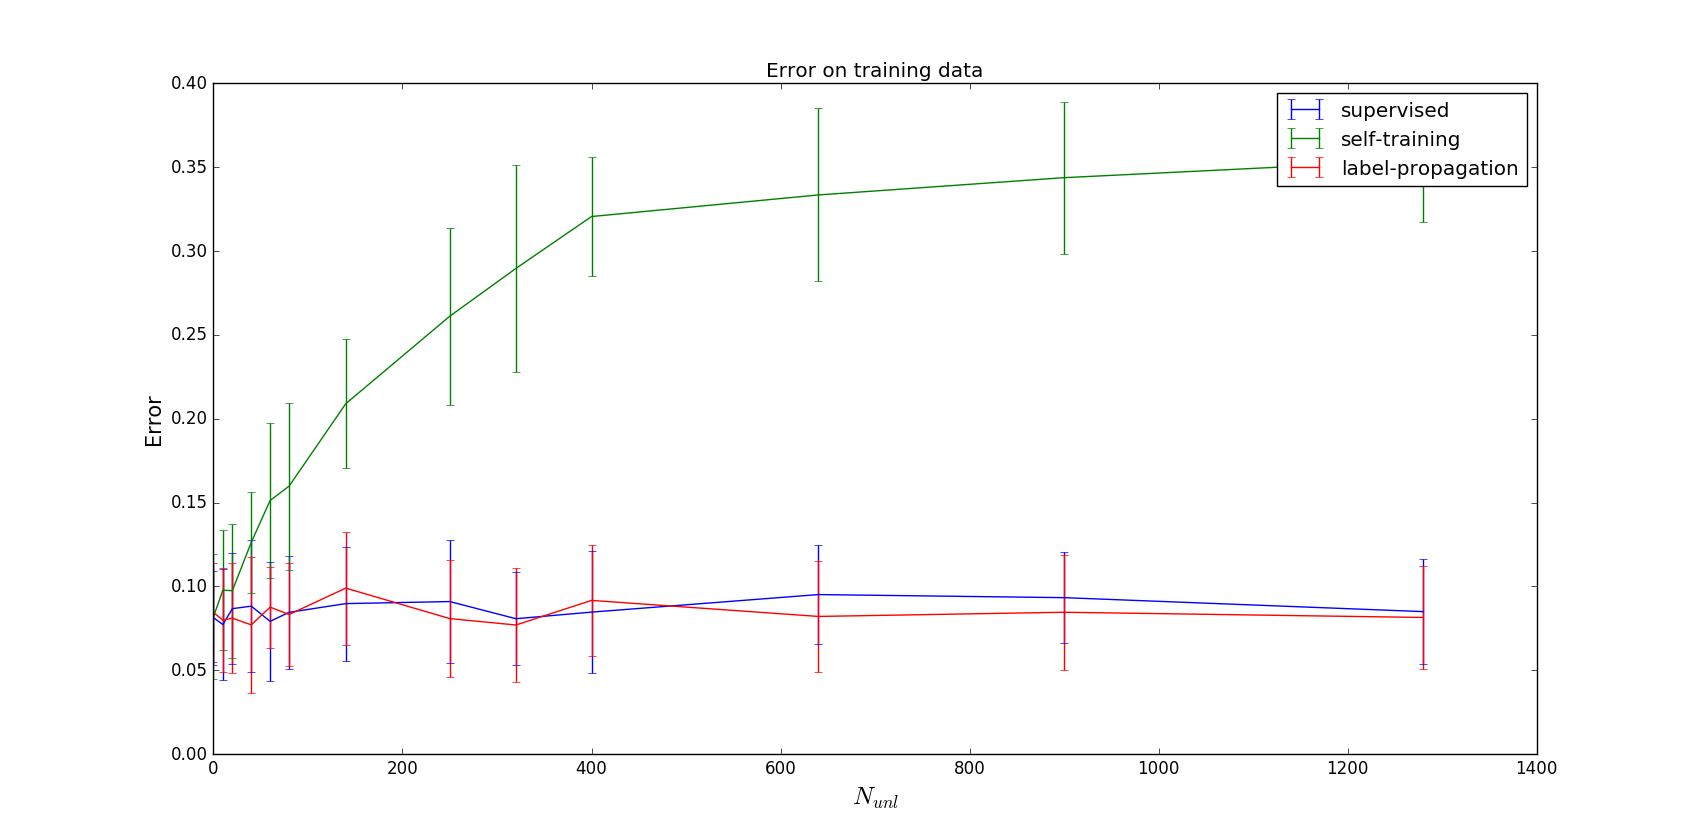
\includegraphics[scale=0.3]{Images/custom1_train_error.png}
			\caption{Training error on the first custom distribution versus number of unlabelled samples, for various implementations of semi-supervised LDA.}
			\label{custom_1}
		\end{center}
	\end{figure}
	
	 
	\bibliographystyle{authordate1}
	\begin{bibliography}{ref}
		
	\end{bibliography}

\end{document}